\section*{Задача 2.2}
Дано уравнение $f(x) = 0$. Найти все корни уравнения с заданной точностью $\varepsilon = 10^{-12}$ на указанном отрезке $[a, b]$. Для решения задачи использовать метод Ньютона и метод простых итераций. Сравнить количество итераций, потребовавшихся для достижения заданной точности каждым методом.
\[f(x) = 10^{-\sqrt{x}}- \sin(\pi \sqrt{x})- 0.9,\]
\[x \in [0, 3].\]

\subsection*{Решение}
Найдем отрезки локализации для каждого корня и середины этих отрезков примим за начальные приближения.

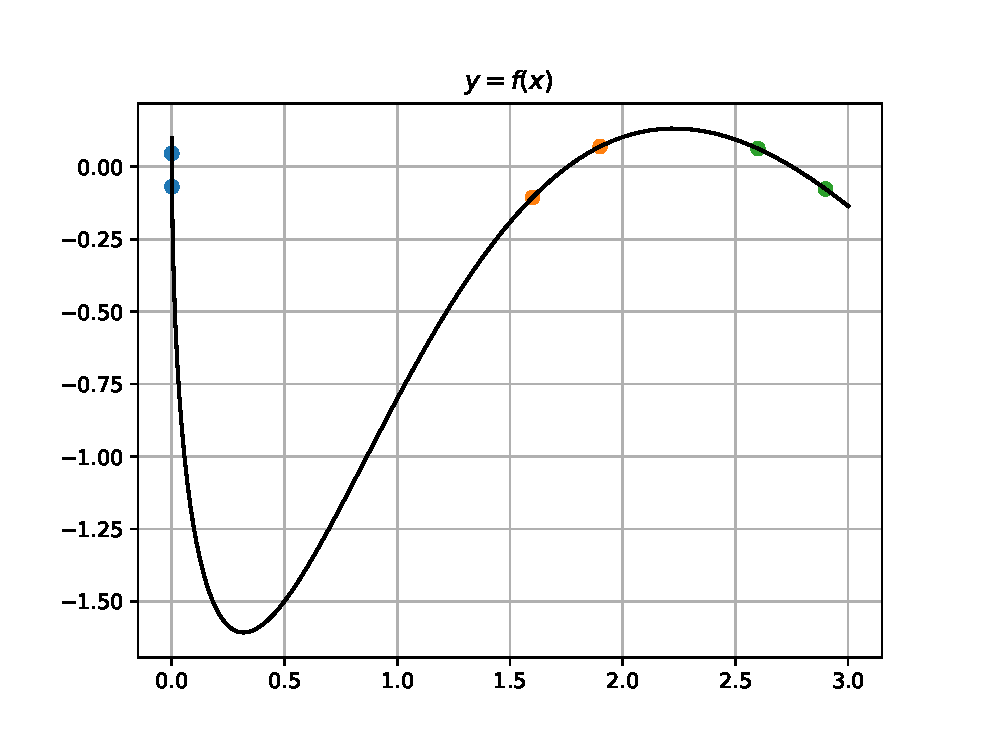
\includegraphics[width=\textwidth]{221.eps}

Составим программу вычисления корня методом Ньютона, предусмотрев в ней подсчёт числа итераций. Найдем с заданной точностью корни уравнения на отрезке $[0, 3]$.

\begin{verbatim}
def newton(x0, func, dfunc, eps):
    x1 = x0 - func(x0) / dfunc(x0)
    it = 1
    while abs(x1 - x0) > eps:
        x0 = x1
        x1 = x0 - func(x0) / dfunc(x0)
        # print(f"\t{x1}")
        it += 1
    print(f"\tВыполнено {it} итераций. x = {x1}")
    return x1
\end{verbatim}

Результаты для каждого из отрезков локализации:
\begin{verbatim}
Выполнено 5 итераций. x = 0.000343705625
Выполнено 4 итераций. x = 1.755702317447
Выполнено 4 итераций. x = 2.751734381135
\end{verbatim}

Составим программу вычисления корня методом простых итераций, предусмотрев в ней подсчёт числа итераций. Найдем с заданной точностью те же корни уравнения.
\begin{verbatim}
def MPI(x0, m1, M1, f, eps):
    alpha = 2 / (m1 + M1)
    q = abs((M1-m1)/ (M1 + m1))
    x1 = x0 - alpha * f(x0)
    it = 1
    while abs(x1 - x0) > (1 - q) * eps / q:
        x0 = x1
        x1 = x0 - alpha * f(x0)
        it += 1
    print(f"\tВыполнено {it} итераций. x = {x1}")
    return x1
\end{verbatim}
Результаты для каждого из отрезков локализации:
\begin{verbatim}
Выполнено 13 итераций. x = 0.000343705625
Выполнено 7 итераций. x = 1.755702317447
Выполнено 7 итераций. x = 2.751734381135
\end{verbatim}

Полученные результаты запишем в таблицу:

{
\centering
\bgroup
\def\arraystretch{1.5}%
\begin{tabular}{|llll|}
\hline
\multicolumn{4}{|l|}{$f(x) = 10^{-\sqrt{x}}- \sin(\pi \sqrt{x})- 0.9$}                                                                                                                                                                                              \\ \hline
\multicolumn{4}{|l|}{Расчетная формула метода Ньютона: $x_{n+1} = x_n - \dfrac{f(x_n)}{f'(x_n)}$}                                                                                                                                                                   \\ \hline
\multicolumn{4}{|l|}{Расчетная формула метода простых итераций: $x_{n+1} = x_n - \alpha f(x_n)$}                                                                                                                                                                    \\ \hline
\multicolumn{4}{|l|}{Задача 2.2}                                                                                                                                                                                                                                    \\ \hline
\multicolumn{1}{|l|}{Начальное приближение} & \multicolumn{1}{l|}{Корень уравнения} & \multicolumn{1}{l|}{\begin{tabular}[c]{@{}l@{}}Число итераций\\ Метод Ньютона\end{tabular}} & \begin{tabular}[c]{@{}l@{}}Число итераций\\ Метод простых итераций\end{tabular} \\ \hline
\multicolumn{1}{|l|}{0.00055}               & \multicolumn{1}{l|}{0.00034370562}    & \multicolumn{1}{l|}{5}                                                                      & 13                                                                              \\ \hline
\multicolumn{1}{|l|}{1.75}                  & \multicolumn{1}{l|}{1.755702317447}   & \multicolumn{1}{l|}{4}                                                                      & 7                                                                               \\ \hline
\multicolumn{1}{|l|}{2.75}                  & \multicolumn{1}{l|}{2.751734381135}   & \multicolumn{1}{l|}{4}                                                                      & 7                                                                               \\ \hline
\end{tabular}
\egroup
}

Модифицируем методы так, чтобы каждый метод делал заданное количество итераций и на каждом шаге сохранял значение модуля невязки $r_n = |f(x_n)|$.
\begin{verbatim}
def newton2(x0, func, dfunc, n, eps):
    x1 = x0 - func(x0) / dfunc(x0)
    r = [abs(f(x1))]
    it = 1
    while it < n:
        x0 = x1
        x1 = x0 - func(x0) / dfunc(x0)
        r.append(abs(f(x1)))
        it += 1
    return x1, np.array(r)

def MPI2(x0, m1, M1, f, n, eps):
    alpha = 2 / (m1 + M1)
    q = abs((M1-m1)/ (M1 + m1))
    x1 = x0 - alpha * f(x0)
    r = [abs(f(x1))]
    it = 1
    while it < n:
        x0 = x1
        x1 = x0 - alpha * f(x0)
        r.append(abs(f(x1)))
        it += 1
    return x1, np.array(r)
\end{verbatim}

Для каждого начального приближения вызовем модифицированные методы так, чтобы они проделали 10 итераций. Построим графики зависимости $r_n$ от $n$ в логарифмической шкале.

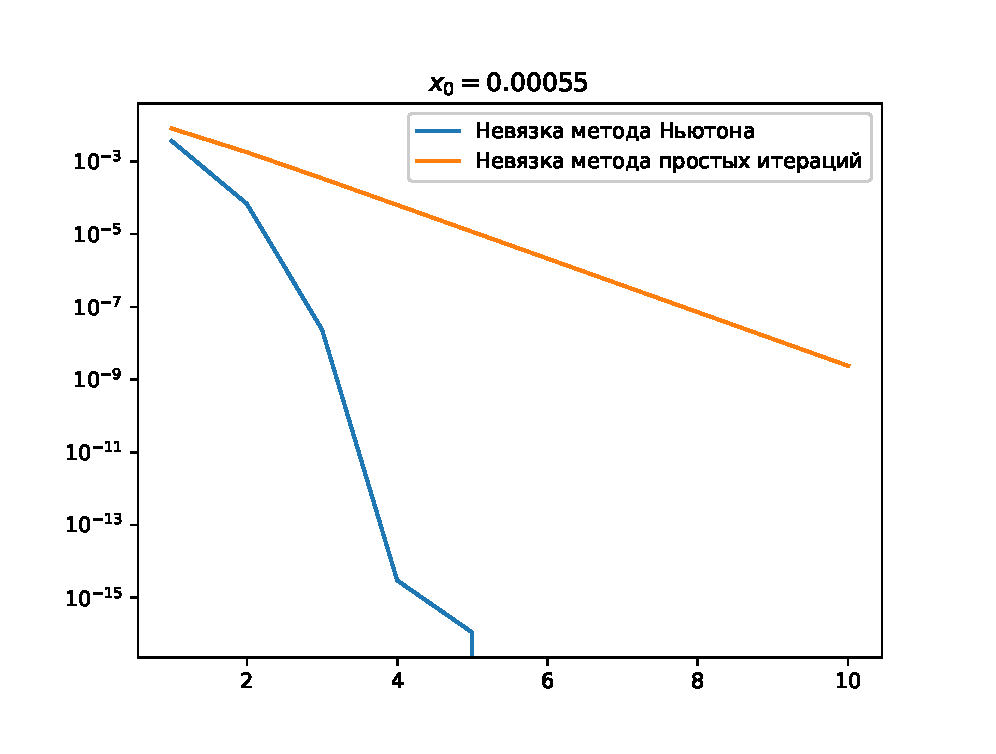
\includegraphics[width=12cm]{222_0.eps}

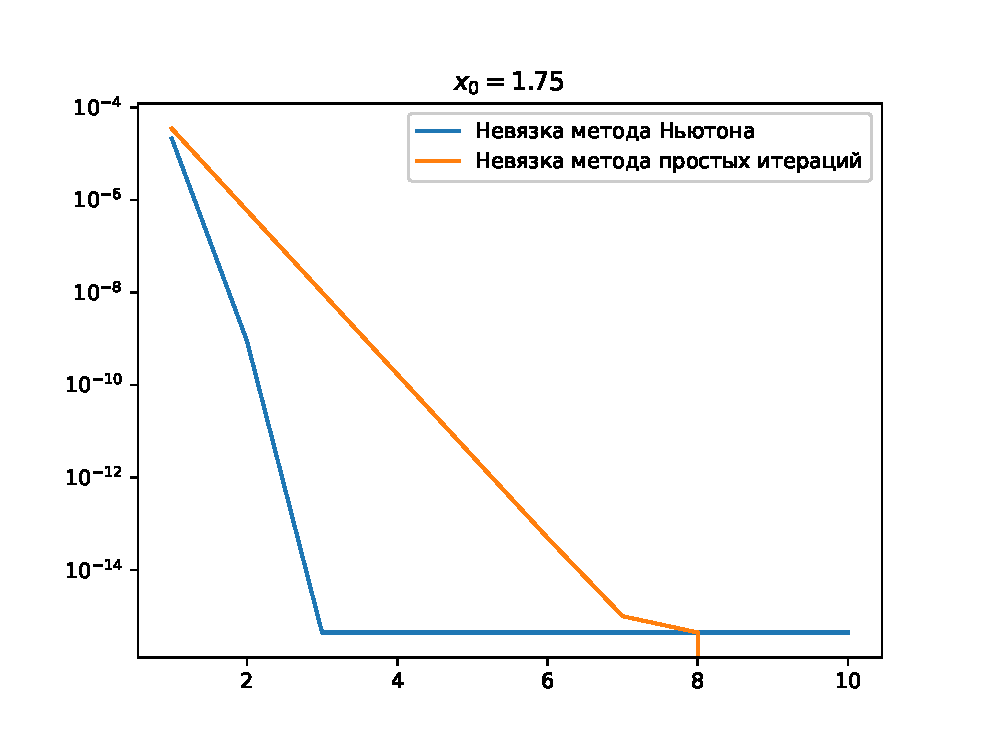
\includegraphics[width=12cm]{222_1.eps}

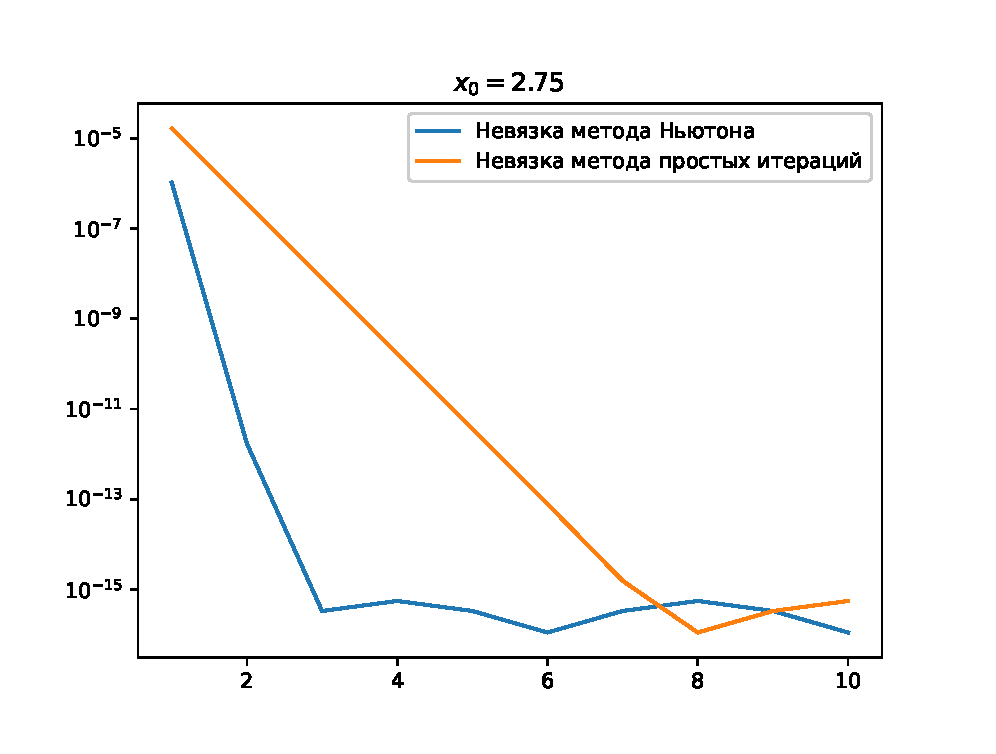
\includegraphics[width=12cm]{222_2.eps}

По полученым графикам можно сделать следующий вывод:

1. Возможно приблизительно определить порядок сходимости методов: для метода Ньютона он равен 2, для метода простых итераций $~1.6$.

2. Больший порядок сходимости позволяет методу быстрее приближаться к точному значению корня, что соответствует теоретическим результатам.

3. Невязка не будет стремиться к нулю из-за погрешности округления значений в памяти компьютера, а также из-за наличия интервала неопределенности корня.

4. Возможно, что начиная с какой-то итерации невязка будет равна нулю (1 график), если компьютер позволяет сохранить точное значение данного корня в памяти.
